An important question arises after introducing a thermal driving force; namely how large (or rather {\it{small}}) is the actual displacement of the vibrating membrane at room and cryogenic temperatures? The membrane fluctuates around zero displacement (equlibrium position) with variance $\langle x^2 \rangle$ due to the random nature of Langevin force $F_{th}$. We will calculate the root mean square displacement $x_{RMS} = \sqrt{\langle x^2 \rangle}$ and from the mechanical power spectral density using Parseval's theorem

\begin{equation}
\begin{split}
\langle x^2 \rangle & = \frac{1}{2\pi}\int_{-\infty}^{\infty}d\Omega S_{xx}(\Omega) \\
 & = \frac{1}{\pi}\frac{k_BT\Gamma_m}{\Omega_{m}^2m_{eff}}\int_{0}^{\infty}d\Omega\left[ \Delta^2 + (\Gamma_m/2)^2 \right]^{-1} \\
 & = \frac{k_BT}{\Omega_{m}^2m_{eff}} \label{eq:t_eff}.
\end{split}
\end{equation}
\noindent
Where we have inserted equation \eqref{eq:full_psd} in the integral and changed the interval of the integration from $-\infty \to 0$ and applied a factor of 2 to compensate. The integral can be solved using \cite{spiegel1999}

\begin{equation}
\int_{0}^{\infty}dx\left[x^2 + a^2 \right]^{-1} = \frac{\pi}{2a}.
\end{equation}
\noindent
Fortunately we end up confirming that this kind of thermal noise gives the equipartition theorem $m_{eff}\Omega_{m}^2\langle x^2 \rangle = k_BT$, which states that the average potential energy is equal to $k_BT/2$ at thermal equilibrium . This is a nice sanity check to see if we made any mistakes so far. Finally, we can write the expression for the root mean square displacement by taking the square root

\begin{equation}
x_{RMS} = \sqrt{\frac{k_BT}{\Omega_{m}^2m_{eff}}}.
\label{eq:rms}
\end{equation}
\noindent
We can find the effective temperature of the membrane from its spectrum, by taking the area underneath the mechanical resonance peak as shown in figure \ref{fig:mem_temp}.

\begin{figure}[H]
\centering
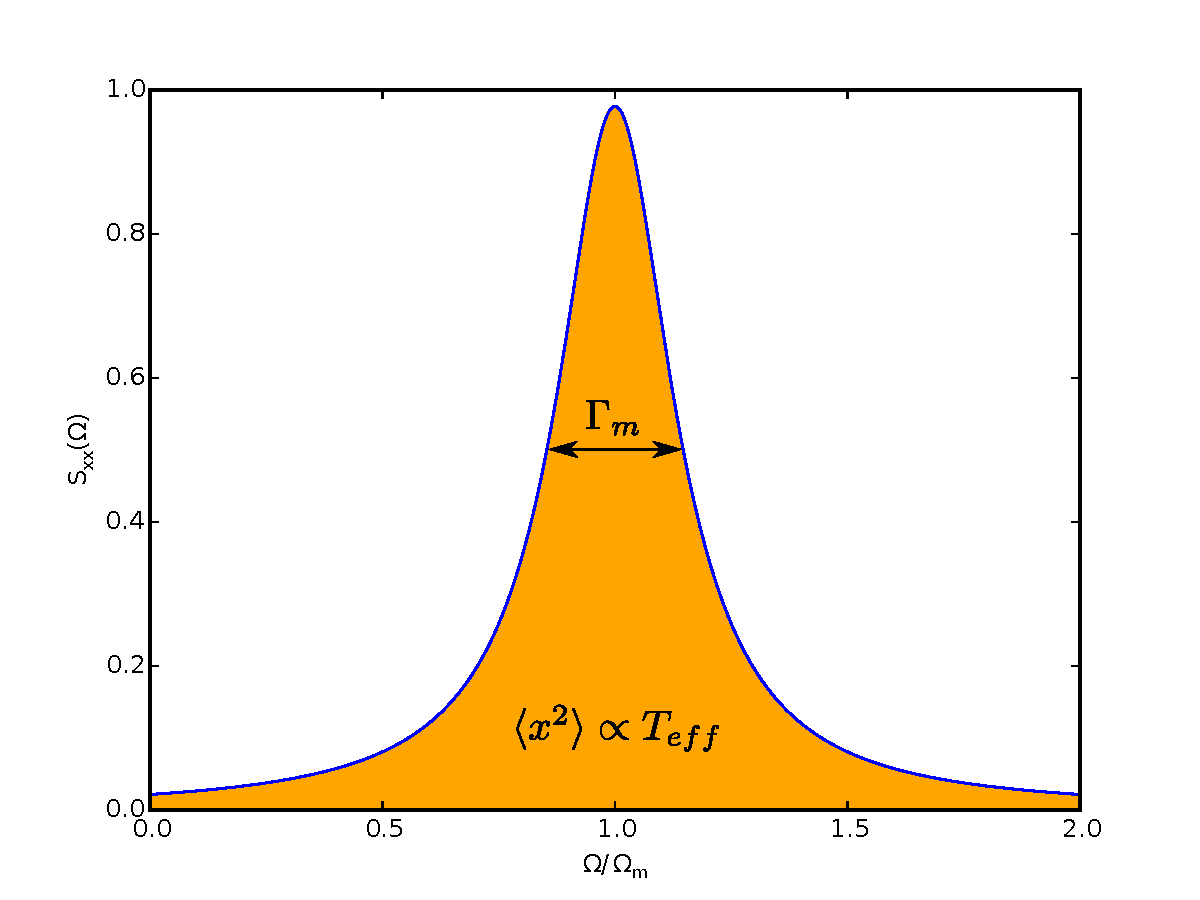
\includegraphics[scale=0.6]{rms.pdf}
\caption{Normalized Lorentzian line shape, representing the mechanical resonance, where $\Gamma_m$ is the width and the area is proportional to the membrane effective temperature $T_{eff}$.}
\label{fig:mem_temp}
\end{figure}

Let us end this chapter by calculating the root mean square displacement for the fundamental mechanical mode at typical working temperatures, i.e. room temperature (\SI{300}{\kelvin}) and cryogenic (liquid helium) typical temperature \SI{4.2}{\kelvin}.

\begin{table}[H]
\centering
\begin{tabular}{ccc}
\toprule
$k_B$ & Boltzmann constant & \SI{1.4e-23}{\square\meter\kilogram\per\square\second\per\kelvin} \\
$T_{room}$ & Temperature & \SI{300.0}{\kelvin} \\
$T_{cryo}$ & Temperature & \SI{4.2}{\kelvin} \\
$\Omega_{1,1}$ & Angular frequency & \SI[product-units=single]{2\pi x 732.0e3}{\radian\per\second} \\
$m_{eff}$ & Effective mass & \SI{10.5}{\nano\gram} \\
\midrule
$x_{RMS_{room}}$ & RMS displacement & \SI{4.3}{\pico\meter} \\
$x_{RMS_{cryo}}$ & RMS displacement & \SI{0.5}{\pico\meter} \\
\bottomrule
\end{tabular}
\caption{Typical membrane properties, normal working temperatures and estimated root mean square displacement.}
\label{tab:RMS_displacement}
\end{table}

From equation \eqref{eq:rms} it follows that as the temperature tends to zero so does the RMS-displacement of the membrane. However, we know from quantum mechanics that this is not completely true, because of quantum fluctuations.